\documentclass[conference]{IEEEtran}
\IEEEoverridecommandlockouts
% The preceding line is only needed to identify funding in the first footnote. If that is unneeded, please comment it out.
\usepackage{cite}
\usepackage{amsmath,amssymb,amsfonts}
\usepackage{algorithmic}
\usepackage{graphicx}
\usepackage{textcomp}
\usepackage{xcolor}
\def\BibTeX{{\rm B\kern-.05em{\sc i\kern-.025em b}\kern-.08em
    T\kern-.1667em\lower.7ex\hbox{E}\kern-.125emX}}
\begin{document}

\title{Detecção de fraudes em transações financeiras usando redes neurais profundas\\
}

\author{\IEEEauthorblockN{1\textsuperscript{st} João Luís da Silva Marrocos}
\IEEEauthorblockA{\textit{Centro de Informática} \\
\textit{Universidade Federal de Pernambuco}\\
Recife, Brasil \\
jlsm2@cin.ufpe.br}
}

\maketitle

\section{Introdução e objetivo}

Com o aumento exponencial das transações financeiras digitais e o crescente uso de cartões de crédito em todo o mundo, a detecção de fraudes financeiras se tornou uma preocupação fundamental para instituições financeiras, comerciantes e consumidores. Transações fraudulentas não apenas causam perdas financeiras, mas também prejudicam a confiança do público nos sistemas de pagamento digital. Dessa forma, a detecção eficaz de fraudes torna-se essencial para manter a segurança e a integridade das operações financeiras.

Os métodos tradicionais de detecção de fraudes baseados em regras fixas e análise manual são frequentemente insuficientes diante da sofisticação crescente dos métodos de fraudes. Por isso, modelos baseados em aprendizado de máquina e redes neurais profundas surgiram como soluções promissoras. Esses modelos têm a capacidade de identificar padrões complexos em grandes volumes de dados, permitindo a detecção de fraudes em tempo real e com maior precisão.

Este projeto foca na detecção de fraudes em transações de cartão de crédito utilizando redes neurais profundas, como redes neurais multi-layer perceptron (MLP) e redes neurais recorrentes (RNNs). O objetivo é desenvolver modelos capazes de diferenciar com precisão transações fraudulentas e legítimas em um grande volume de dados financeiros. Para isso, apliquei técnicas avançadas de balanceamento de dados, como o SMOTE, para lidar com a natureza desbalanceada dos dados de fraudes, além de realizar um extenso pré-processamento para garantir a qualidade dos dados de entrada.

\section{Metodologia}

A metodologia deste projeto segue um fluxo estruturado de etapas, desde o pré-processamento dos dados até o treinamento e avaliação de modelos baseados em redes neurais profundas. O processo pode ser dividido em quatro fases principais: escolha do \textit{dataset} e preparação de dados, pré-processamento, treinamento de modelos e avaliação de desempenho.

\subsection{\textit{Dataset}}

O \textit{dataset} selecionado no site \textit{Kaggle} na verdade conta com dois arquivos \textit{.csv} devidamente divididos em dados de teste e dados de treino, o que facilitou bastante na etapa de separação entre dados de teste e de treino para o treinamento dos modelos. O conjunto de dados conta com diversas colunas (\textit{features}) que são úteis para identificar e classificar se há fraude ou não:

\begin{itemize}
    \item \textbf{index} - Identificador único para cada linha
    \item \textbf{trans\_date\_trans\_time} - Data e hora da transação
    \item \textbf{cc\_num} - Número do cartão de crédito do cliente
    \item \textbf{merchant} - Nome do comerciante
    \item \textbf{category} - Categoria do comerciante
    \item \textbf{amt} - Valor da transação
    \item \textbf{first} - Primeiro nome do titular do cartão de crédito
    \item \textbf{last} - Sobrenome do titular do cartão de crédito
    \item \textbf{gender} - Gênero do titular do cartão de crédito
    \item \textbf{street} - Endereço do titular do cartão de crédito
    \item \textbf{city} - Cidade do titular do cartão de crédito
    \item \textbf{state} - Estado do titular do cartão de crédito
    \item \textbf{zip} - Código postal do titular do cartão de crédito
    \item \textbf{lat} - Localização em latitude do titular do cartão de crédito
    \item \textbf{long} - Localização em longitude do titular do cartão de crédito
    \item \textbf{city\_pop} - População da cidade do titular do cartão de crédito
    \item \textbf{job} - Profissão do titular do cartão de crédito
    \item \textbf{dob} - Data de nascimento do titular do cartão de crédito
    \item \textbf{trans\_num} - Número da transação
    \item \textbf{unix\_time} - Hora da transação em formato UNIX
    \item \textbf{merch\_lat} - Localização em latitude do comerciante
    \item \textbf{merch\_long} - Localização em longitude do comerciante
    \item \textbf{is\_fraud} - Indicador de fraude \textless--- Classe alvo
\end{itemize}

Ao todo, o conjunto de dados de treino possui aproximadamente 1.3 milhões de linhas e o conjunto de dados de teste possui aproximadamente 550 mil linhas, ambos contendo as mesmas \textit{features}.

\subsection{Processamento dos dados}

Essa etapa do processo é extremamente importante para que os modelos consigam atuar de maneira correta, seguindo um passo a passo para garantir que tudo será feito de forma eficiente:

\begin{itemize}
    \item Remoção de colunas irrelevantes: colunas contendo \textit{features} como: número da transação, número do cartão de crédito, nome do comprador e data de nascimento do comprador foram removidas por não serem úteis para a identificação de fraude, ou por serem dados sensíveis que poderiam enviesar os modelos.

    \item Verificando a existência de valores nulos: valores ausentes (NaN) foram identificados e removidos do dataset, uma vez que a presença de deles pode interferir nas análises subsequentes e no desempenho dos modelos.

    \item Conversão de colunas de data: colunas contendo datas como a "\textit{trans\_date\_trans\_time}" foram convertidas de texto para data utilizando uma ferramenta da biblioteca \textit{Pandas}.

    \item Balanceamento do \textit{dataset}: conjuntos de dados contendo casos de fraudes financeiras naturalmente possuem um desbalanceamento entre os casos que são fraude e os que não são. No \textit{dataset} utilizado, há uma proporção de 99\% de casos que não haviam fraude para 1\% que realmente tinham. Esse desbalanceamento acaba por atrapalhar no treinamento dos modelos, uma vez que se os mesmos julgarem fraude em 100\% dos casos, ainda terão 99\% de acurácia na análise do seu desempenho, o que não é ideal. Então, foi utilizado uma técnica de \textit{oversampling} chamada SMOTE(Synthetic Minority Over-sampling Technique) para balancear o \textit{dataset} corretamente.

    \item Padronização de features numéricas: a padronização das features numéricas é crucial para garantir que os modelos funcionem corretamente, permitindo uma melhor convergência e desempenho, além de facilitar a comparação entre diferentes características.
\end{itemize}

\subsection{Redes neurais profundas utilizadas}

Nesse projeto, optei por utilizar e testar duas redes neurais profundas: LSTM (Long Short-Term Memory) e MLP (Multi Layer Perceptron) e analisar qual se adequaria melhor.

\subsubsection{Long Shot-Term Memory}

\indent A Long Short-Term Memory (LSTM) é um tipo de rede neural recorrente (RNN) projetada para processar sequências de dados. Ao contrário das RNNs tradicionais, que sofrem com o problema do desvanecimento do gradiente, as LSTMs são capazes de aprender dependências de longo prazo de maneira eficaz.

\begin{figure}[h!]
    \centering
    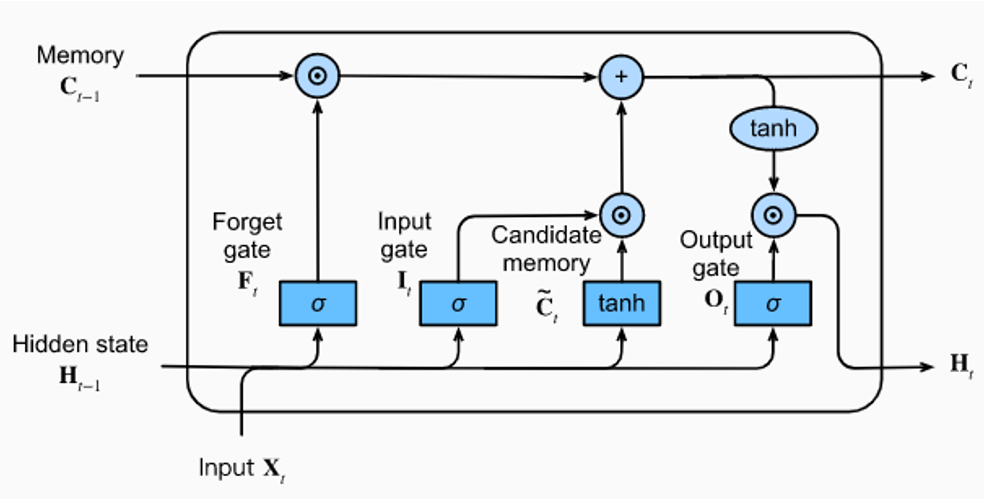
\includegraphics[width=\linewidth]{lstm.png}
    \caption{Estrutura da LSTM}
    \label{fig:lstm}
\end{figure}

\indent A estrutura de uma LSTM conta com Unidades de Memória que podem reter informações ao longo de várias iterações. Isso permite que elas captem padrões e dependências que estão distantes no tempo. Além de 3 portas de controle: a porta de esquecimento que decide quais informações antigas devem ser esquecidas, a porta de entrada que controla quais novas informações devem ser armazenadas na célula e a porta de saída que define quais informações devem ser usadas para a saída atual.

\subsubsection{Multi-Layer Perceptron}

\indent A Multi-Layer Perceptron (MLP) é um tipo de rede neural artificial totalmente conectada, formada por múltiplas camadas de neurônios. É uma das arquiteturas mais básicas de redes neurais feedforward, em que a informação flui em uma única direção, da entrada para a saída, sem ciclos.

\begin{figure}[h!]
    \centering
    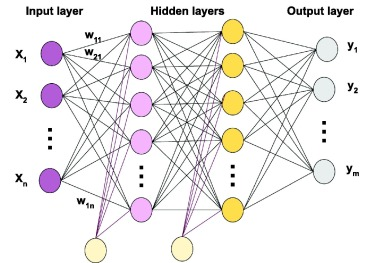
\includegraphics[width=\linewidth]{mlp.jpg}
    \caption{Estrutura da MLP}
    \label{fig:mlp}
\end{figure}


\indent A estrutura da MLP é composta por uma camada de entrada que recebe os dados de entrada, camadas ocultas (\textit{hidden layers}) que são camadas que transformam a entrada aplicando funções de ativação não-lineares e uma camada de saída que produz a previsão final ou classificação do modelo.

\section{Resultados}

Os resultados obtidos ao longo deste projeto evidenciam a eficiência dos modelos de redes neurais profundas na classificação de fraude em transações financeiras. A análise detalhada dos dados, juntamente com a implementação e o treinamento adequados dos modelos, resultou em um desempenho relevante na detecção de fraudes. Nesta seção, serão discutidos os resultados dos modelos utilizados no projeto: LSTMs e MLPs.

\subsection{Long Short-Term Memory}

Para o treinamento do modelo LSTM, primeiramento os dados tiveram que ser redimensionados e transformados em \textit{tensors}. Isso serve para que o modelo consiga ser treinado de forma correta, visto que a bilbioteca \textit{Pytorch} exige que os dados estejam nesse formato.

Os hiperparâmetros utilizados foram:

\begin{itemize}
    \item \textbf{Tamanho da Entrada (input\_size)}: Define o número de features (características) de cada amostra de entrada. No código, esse valor é definido como \texttt{X\_train.shape[2]}, ou seja, o número de colunas no conjunto de dados de entrada.
    
    \item \textbf{Tamanho da Camada Oculta (hidden\_size)}: Número de neurônios na camada oculta da LSTM. No código, o valor foi definido como 64, representando a quantidade de unidades ocultas: \texttt{self.lstm = nn.LSTM(input\_size, 64, batch\_first=True, dropout=0.5)}.
    
    \item \textbf{Dropout}: Taxa de dropout utilizada para regularizar o modelo e prevenir overfitting. No código, o valor é 0.5: \texttt{dropout=0.5}.
    
    \item \textbf{Tamanho da Saída (output\_size)}: O tamanho da saída da camada totalmente conectada é 1, pois o problema é de classificação binária (fraude ou não fraude): \texttt{self.fc = nn.Linear(64, 1)}.
    
    \item \textbf{Função de Ativação (Sigmoid)}: A função de ativação usada na última camada é a Sigmoid, que converte a saída do modelo em um valor entre 0 e 1 para a classificação binária: \texttt{self.sigmoid = nn.Sigmoid()}.
    
    \item \textbf{Taxa de Aprendizado (learning rate)}: A taxa de aprendizado usada pelo otimizador Adam foi definida como 0.001: \texttt{lr=0.001}.
    
    \item \textbf{Função de Perda (loss function)}: A função de perda utilizada é a \texttt{Binary Cross Entropy Loss (BCELoss)}, apropriada para classificação binária.
\end{itemize}

O treinamento foi feito em 10 épocas e teve resultados interessantes com as métricas utilizadas:

\begin{figure}[h!]
    \centering
    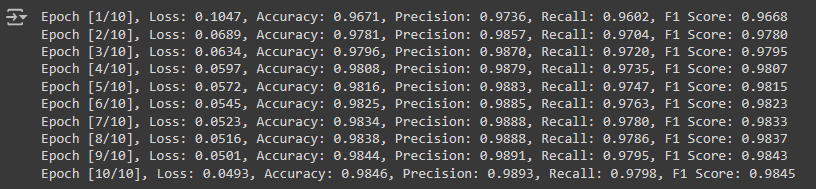
\includegraphics[width=\linewidth]{lstm-results.png}
    \caption{Resultados LSTM}
    \label{fig:result-lstm}
\end{figure}

O modelo apresentou uma acurácia de aproximadamente 98\% durante o treinamento, o que se deve bastante ao pre-processamento correto dos dados.

\subsection{Multi-Layer Perceptron}

De forma semelhante a LSTM, os dados tiveram que ser redimensionados e transformados em \textit{tensors}, para que a ferramenta de treinamento tratasse eles da forma correta.

Os hiperparametros utilizados foram:

\begin{itemize}
    \item \textbf{Tamanho da Entrada (input\_size)}: Define o número de features (características) de cada amostra de entrada. No código, esse valor é definido como \texttt{X\_train.shape[1]}, que representa o número de colunas no conjunto de dados de entrada.
    
    \item \textbf{Número de Neurônios na Primeira Camada Oculta}: O número de neurônios na primeira camada oculta é 128, que foi definido no código como \texttt{self.fc1 = nn.Linear(input\_size, 128)}.
    
    \item \textbf{Número de Neurônios na Segunda Camada Oculta}: O número de neurônios na segunda camada oculta é 64, definido como \texttt{self.fc2 = nn.Linear(128, 64)}.
    
    \item \textbf{Número de Neurônios na Terceira Camada Oculta}: O número de neurônios na terceira camada oculta é 32, especificado como \texttt{self.fc3 = nn.Linear(64, 32)}.
    
    \item \textbf{Função de Ativação (ReLU)}: A função de ativação utilizada nas camadas ocultas é a ReLU (Rectified Linear Unit), que é aplicada como \texttt{self.relu = nn.ReLU()}.
    
    \item \textbf{Função de Ativação da Camada de Saída (Sigmoid)}: A função de ativação na camada de saída é a Sigmoid, que converte a saída do modelo em um valor entre 0 e 1, apropriada para classificação binária: \texttt{self.sigmoid = nn.Sigmoid()}.
    
    \item \textbf{Taxa de Aprendizado (learning rate)}: A taxa de aprendizado usada pelo otimizador Adam foi definida como 0.001: \texttt{lr=0.001}.
    
    \item \textbf{Função de Perda (loss function)}: A função de perda utilizada é a \texttt{Binary Cross Entropy Loss (BCELoss)}, que é adequada para problemas de classificação binária.
\end{itemize}

\begin{figure}[h!]
    \centering
    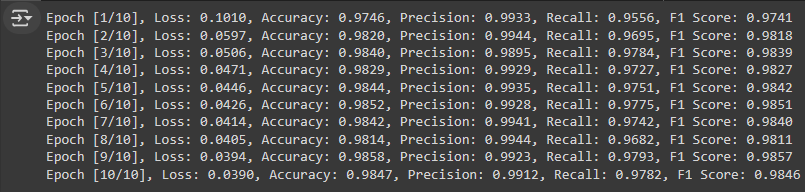
\includegraphics[width=\linewidth]{mlp-results.png}
    \caption{Resultados MLP}
    \label{fig:result-mlp}
\end{figure}

Durante o treinamento do modelo, foi possivel observar uma acurácia média de 98\%, um desempenho muito semelhante ao do modelo LSTM.

\section{Conclusão e considerações finais}

Apesar dos dois modelos terem apresentado desempenhos muito semelhantes, o modelo MLP se sobressaiu por ter um tempo de treinamento ligeiramente menor. Enquanto o tempo de treinamento das 10 épocas do modelo MLP ficou em torno dos 25 minutos, o treinamento do modelo LSTM beirou os 40 minutos. Esse tempo elevado de treinamento se deve muito ao tamanho da base de dados escolhida.

É claro que esse desempenho pode mudar de máquina para máquina, então devido à boa performance dos dois modelos, ambos serão muito úteis para a detecção de fraude em transações de cartão de crédito por todo o mundo, ajudando os compradores a evitar esse tipo de empecilho.

\begin{thebibliography}{00}
\bibitem{b1} I. Goodfellow, Y. Bengio, and A. Courville, ``Deep Learning,'' MIT Press, 2016. [Online]. Available: http://www.deeplearningbook.org/

\bibitem{b2} S. Hochreiter and J. Schmidhuber, ``Long short-term memory,'' Neural Computation, vol. 9, no. 8, pp. 1735--1780, 1997. [Online]. Available: https://www.bioinf.jku.at/publications/older/2604.pdf

\bibitem{b3} Z. Pan, Y. Wang, and Y. Zhang, ``Credit card fraud detection using LSTM based deep learning model,'' IEEE Access, vol. 7, pp. 23282--23291, 2019. [Online]. Available: https://ieeexplore.ieee.org/document/8615301

\bibitem{b4} S. Hasan, M. Y. Javed, J. Qadir, I. Khatak, and A. Fatima, ``Real-time credit card fraud detection using machine learning: a survey,'' in Proceedings of the 2016 International Conference on Communication, Computing and Digital Systems (C-CODE), 2016, pp. 105--110. [Online]. Available: https://ieeexplore.ieee.org/document/7578912

\bibitem{b5} S. Li, J. Zhao, and X. Wang, ``Fraud detection in credit card transactions using machine learning: A systematic review,'' Information Systems, vol. 78, pp. 12--25, 2018. [Online]. Available: https://www.sciencedirect.com/science/article/pii/S0306437918302050

\bibitem{b6} A. Gulli and S. Pal, \textit{Deep Learning with Python and PyTorch}, 1st ed. Birmingham: Packt Publishing, 2019.
\end{thebibliography}

\end{document}
